\documentclass{beamer}

\mode<presentation> {
  \usetheme{PaloAlto}
}

%%
\makeatletter
\setbeamertemplate{subsubsection in sidebar}{\vspace*{-\baselineskip}}
\setbeamertemplate{subsubsection in sidebar shaded}{\vspace*{-\baselineskip}}
\makeatother
%%

%%
\setbeamertemplate{theorems}[numbered]
%%

\definecolor{Garnet}{RGB}{130,0,20}
\usecolortheme[named=Garnet]{structure}

\logo{
\includegraphics[width=1.5cm]{../../sharedImgs/USClogo.png}}

%\setbeamercolor{title}{fg=red!60!black,bg=white!50!black}
%\usecolortheme{beaver}
%\usecolortheme{crane}
\usefonttheme{structuresmallcapsserif}
\usefonttheme[onlysmall]{structurebold}

\usepackage{multicol}
\usepackage{graphicx}
\usepackage{mathtools}
\usepackage{latexsym}
\usepackage{amsfonts}
\usepackage[only,ninrm,elvrm,twlrm,sixrm,egtrm,tenrm]{rawfonts}
\usepackage{indentfirst}
\usepackage[noend]{algorithmic}
\usepackage{algorithm}
\usepackage{enumerate}
\usepackage{graphicx,psfrag}
\usepackage{epsfig}
%\usepackage[pdflatex]{graphicx}
%\usepackage{epstopdf}
\usepackage{ulem}
\usepackage{animate} %need the animate.sty file
\usepackage{tikz}
\usetikzlibrary{fit,shapes,calc}
\usepackage{pgfplots}
\usepackage{amsmath,amsthm,amssymb,amsfonts,enumerate,mymath,mathtools,tikz-cd,mathrsfs}

\newtheorem{thm}{Theorem}
\newtheorem{lem}{Lemma}
\newtheorem{prop}{Proposition}
\theoremstyle{definition}
\newtheorem{defn}{Definition}
\newtheorem{rmk}{Remark}

\newcommand{\A}{\mathscr{A}}
\renewcommand{\C}{\mathscr{C}}

\newcommand*{\defeq}{\mathrel{\vcenter{\baselineskip0.5ex \lineskiplimit0pt
                     \hbox{\scriptsize.}\hbox{\scriptsize.}}}%
                     =}
\DeclarePairedDelimiter\ceil{\lceil}{\rceil}
\DeclarePairedDelimiter\floor{\lfloor}{\rfloor}

\input epsf



\usepackage[english]{babel}
% or whatever

\usepackage[latin1]{inputenc}
% or whatever

\usepackage{times}
\usepackage[T1]{fontenc}
% Or whatever. Note that the encoding and the font should match. If T1
% does not look nice, try deleting the line with the fontenc.

\title % (optional, use only with long paper titles)
    {Proportionality and Power Functions}

\author[Farman]
{Blake Farman~\inst{1}}

\institute[USC]{
\inst{1}
University of South Carolina, Columbia, SC USA}
%\inst{2}
%East Carolina University, Greenville, NC USA\\
%\inst{3}
%University of Johannesburg, Auckland Park, South Africa}

\date[January 17, 2017]
{Math 122: Calculus for Business Administration and Social Sciences}

%\subject{Irredundant and Mixed Ramsey Numbers}
\setbeamercolor{alerted text}{fg=red!60!black}
\setbeamercolor{block title}{bg=white!50!black,fg=red!60!black}

\begin{document}

\begin{frame}
  \titlepage
\end{frame}

\begin{frame}
  \frametitle{Outline}
  \tableofcontents[pausesections]
\end{frame}

\section{1.9: Proportionality and Power Functions}
\begin{frame}{Proportionality}
  \begin{defn}
    We say that $y$ is {\it (directly) proportional} to $x$ if there is a non-zero constant $k$ such that 
    $$y = kx.$$
    \onslide<2->{The constant $k$ is called the constant of proportionality.}
  \end{defn}
  
  \onslide<3->{
      \begin{rmk}
        This is a fancy way of saying the function $y(x) = kx$ is a line through the origin.
      \end{rmk}
    }
\end{frame}

\begin{frame}{Example}
  The heart mass of a mammal is proportional to its mass.
  \begin{enumerate}[(a)]
    \item<1->
      Write a function for the heart mass, $H$, in terms of body mass, $B$.
      \onslide<2->{$$H(B) = kB.$$}
    \item<3->
      A human with a body mass of 70 kg has a heart mass of $0.42$ kg.
      Find teh constant of proportionality.
      \begin{eqnarray*}
        \onslide<4->{\frac{42}{100} &=& 70k\\}
        \onslide<5->{\Rightarrow k &=& \frac{42}{7000} \approx 0.006}
      \end{eqnarray*}
      \item<6-> Estimate the heart mass of a horse with body mass of 650 kg.
  \end{enumerate}
\end{frame}

\begin{frame}{Example (Cont.)}
  $$H(650) \approx 0.006(650) \pause = 3.9\ \text{kg}.$$
\end{frame}

\begin{frame}{Power Function}
  \begin{defn}
    We say that $Q(x)$ is a {\it power function} if 
    $$Q(x) = kx^p$$
    for some fixed $k$, $p$.
  \end{defn}
  \onslide<2->{
    \begin{rmk}
      Generally, one calls this a {\it monomial} when $0 \leq p$.
    \end{rmk}
    }
\end{frame}

\subsection{Graphs of Power Functions}

\begin{frame}{$x^{2n}$}
  \begin{center}
  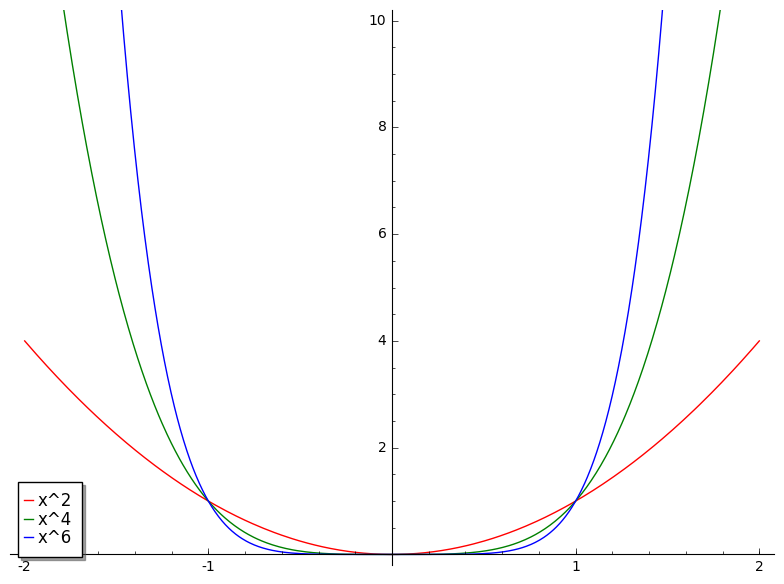
\includegraphics[scale=0.5]{imgs/power1.png}
  \end{center}
\end{frame}

\begin{frame}{$x^{2n + 1}$}
  \begin{center}
    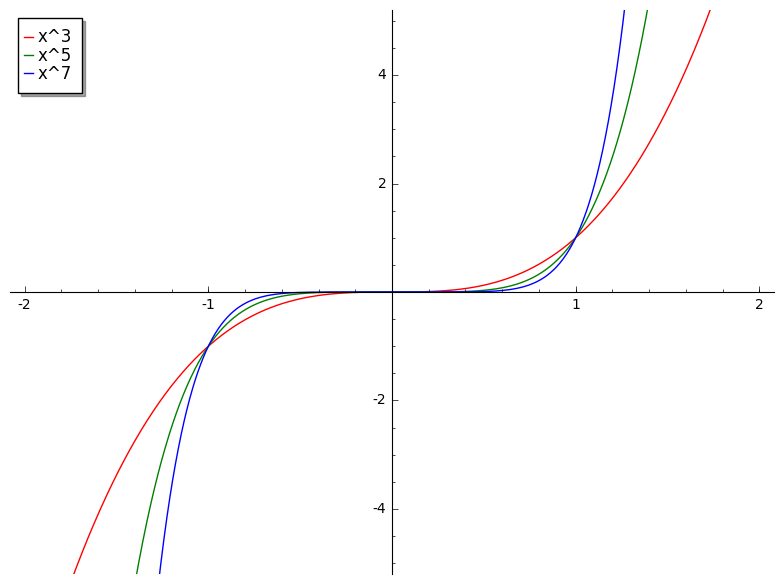
\includegraphics[scale=0.5]{imgs/power2.png}
  \end{center}
\end{frame}

\begin{frame}{$\sqrt[2n]{x}$}
  \begin{center}
    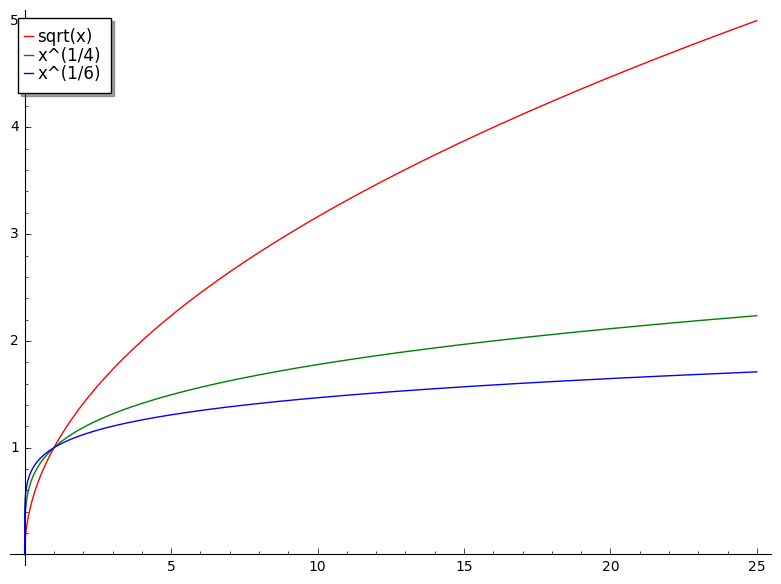
\includegraphics[scale=0.5]{imgs/power3.png}
  \end{center}
\end{frame}

\begin{frame}{$\sqrt[2n + 1]{x}$}
  \begin{center}
    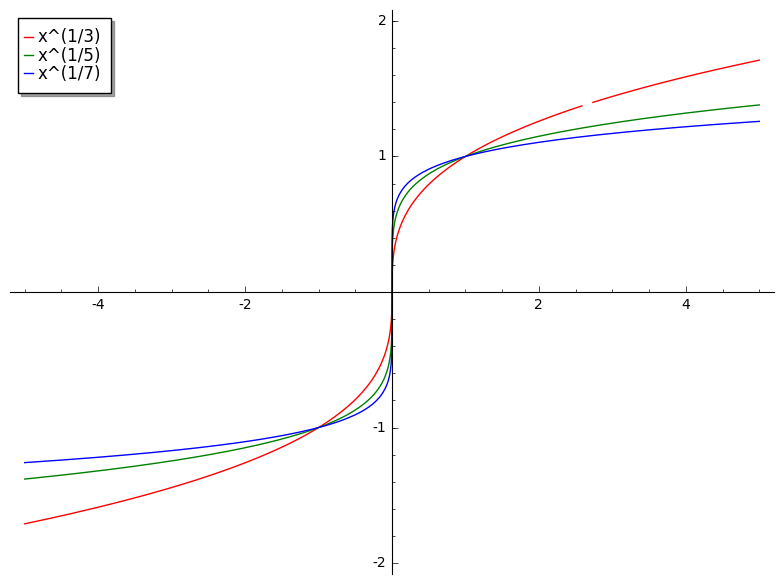
\includegraphics[scale=0.5]{imgs/power4.png}
  \end{center}
\end{frame}

\begin{frame}{$x^{-2n}$}
  \begin{center}
    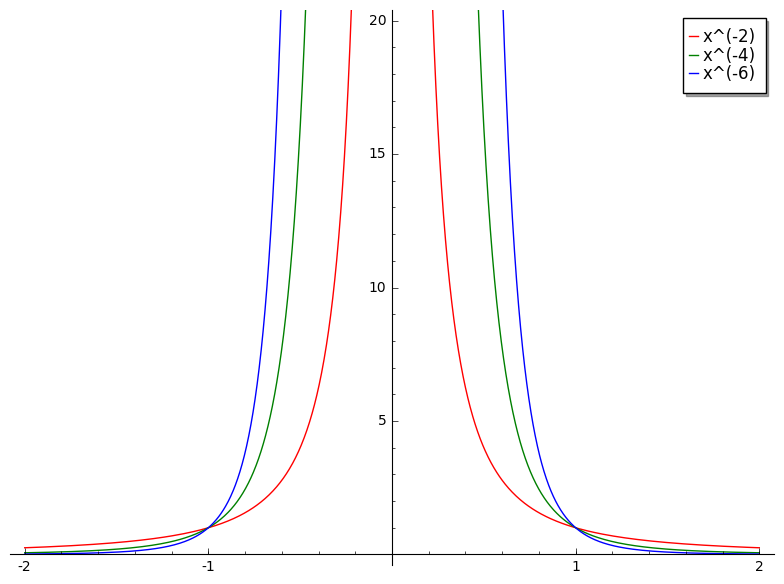
\includegraphics[scale=0.5]{imgs/power5.png}
  \end{center}
\end{frame}

\begin{frame}{$x^{-(2n + 1)}$}
  \begin{center}
    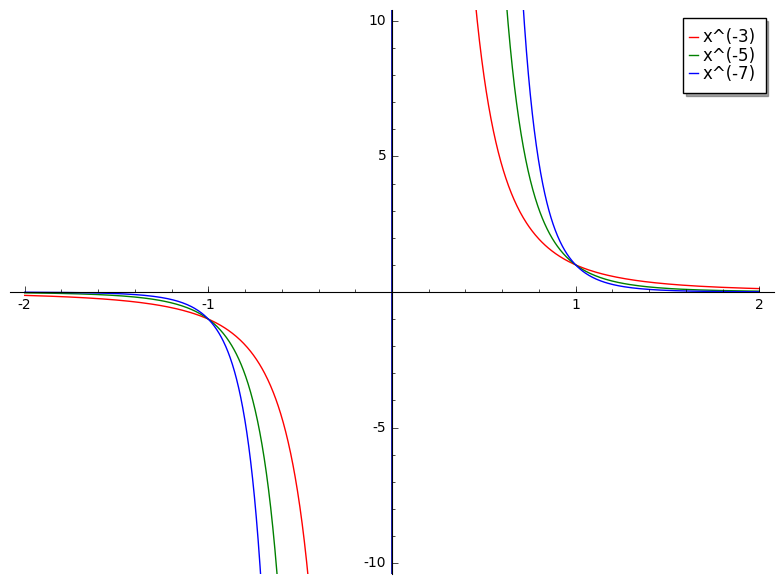
\includegraphics[scale=0.5]{imgs/power6.png}
  \end{center}
\end{frame}

\begin{frame}{Polynomials}
  \begin{defn}
    Sums of power functions with non-negative integer exponents
    $$a_nx^n + a_{n-1}x^{n-1} + \cdots + a_1x + a_0, a_n \neq 0$$
    are {\it polynomials of degree $n$}.
  \end{defn}

  \onslide<2->{
    \begin{rmk}
      When the $n = 2$, one calls the polynomial a {\it quadratic}
  \end{rmk}
  }
\end{frame}

\subsection{Quadratics}

\begin{frame}{Vertex Form}
  Any quadratic, $f(x) = ax^2 + bx + c$, can be written in vertex form
  $$f(x) = a(x - h)^2 + k,$$
  where $(h,k)$ is the vertex of the parabola.
\end{frame}

\begin{frame}{Vertex Form (Cont.)}
  \begin{eqnarray*}
    ax^2 + bx + c &=& a\left(x^2 + \frac{b}{a}x\right) + c\\
    \onslide<2->{&=& a \left(x^2 + \frac{b}{a} + \left(\frac{b}{2a}\right)^2 - \left(\frac{b}{2a}\right)^2\right) + c\\}
    \onslide<3->{&=& a\left(\left(x + \frac{b}{2a}\right)^2 - \left(\frac{b}{2a}\right)^2\right) + \frac{4ac}{4a}\\}
    \onslide<4->{&=& a\left(x - \frac{-b}{2a}\right)^2 + \frac{4ac - b^2}{4a}}
  \end{eqnarray*}
  \onslide<5->{So $h = -b/2a$ and $k = f(h) = (4ac - b^2)/4a$.}
\end{frame}

\begin{frame}{The Quadratic Formula}
  The solutions to the quadratic equation
  $$ax^2 + bx + c = 0$$
  are given by
  $$x = \frac{-b \pm \sqrt{b^2 - 4ac}}{2a}.$$
\end{frame}

\begin{frame}{Graphing Quadratics}
  \begin{enumerate}
  \item<1->
    Put the quadratic in vertex form,
    $$ax^2 + bx + c = a(x - h)^2 + k.$$
  \item<2->
    Graph the parabola $x^2$.
  \item<3->
    Shift horizontally by $h$.
  \item<4->
    Stretch vertically by $\abs{a}$ and reflect across the $x$-axis if $a < 0$.
  \item<5->
    Translate vertically by $k$.
  \end{enumerate}
\end{frame}

\begin{frame}{Example}
  \begin{itemize}
    \item<1->
      A company finds that the average number of people attending a concert is 75 if the price is $\$50$.
    \item<2->
      At a price of $\$35$ per person, the average number of people attending is 120.
  \end{itemize}
  \onslide<3->{Determine the price that will generate the greatest revenue assuming the number of people attending a concert is a linear function of the price.}
\end{frame}

\begin{frame}{Example (Cont.)}
  Assuming the relationship is linear, the slope of the quantity function is
  $$\onslide<2->{m = \frac{120 - 75}{35 - 50}} \onslide<3->{= \frac{45}{-15}} \onslide<4->{= -3}$$
  \onslide<5->{so the quantity of people attending a concert at price $p$ is}
  $$\onslide<6->{q - 75 = -3(p - 50)} \onslide<7->{\Rightarrow q(p) = -3p + 225}$$
  \onslide<8->{Hence the revenue is}
  $$\onslide<8->{R(p) = p\cdot q(p)} \onslide<9->{ = p(-3p + 225)} \onslide<10->{ = -3p^2 + 225p}.$$
\end{frame}

\begin{frame}{Example (Cont.)}
  \begin{itemize}
    \item<1->
      The roots of $R$ are $p = 0$ and $p = 75$.
    \item<2->
      The $x$-coordinate of the vertex is
      $$\frac{-225}{2(3)} = 37.5$$
    \item<3->
      The $y$-coordinate of the vertex is 
      \begin{eqnarray*}
        \onslide<4->{R(37.5) &=& -3(37.5)(37.5 - 75)\\}
        \onslide<5->{&=& -3(37.5)(-37.5)\\}
        \onslide<6->{&=& 3(37.5)^2\\}
        \onslide<7->{&=& 4,218.75.}
      \end{eqnarray*}
  \end{itemize}
\end{frame}
\begin{frame}
  It's clear from the graph that this is the maximum revenue:
    \begin{center}
      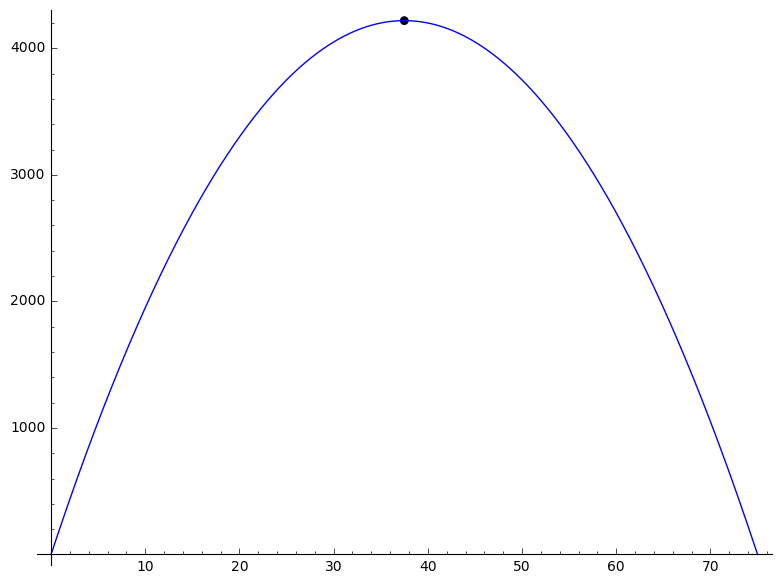
\includegraphics[scale=0.45]{imgs/revenue.png}
    \end{center}
\end{frame}
\end{document}
